\chapter{پیشنیاز های نصب و معرفی قسمت های مختلف}\label{ch:req}

\section{نرم‌افزار‌های کلی}
در این پروژه از جهت آنکه نسخه قبلی و پیشینی برای  آن نبوده است، به ناچار می‌بایست که کد آن از صفر تا صد آن به صورت دستی نوشته شود. از این‌رو، پیچیدگی های بسیار فراوان را به طور خاص در پی داشت. ابزار های زیادی نیز بنابه شرایط در آن استفاده شد که ارتباط بین آن ابزار ها و اجزا، بر این پیچیدگی پیاده سازی طرح افزوده بود.

ابزار های اصلی و کلی که در این پروژه استفاده شده بود، عبارتند از:

\begin{itemize}
	\item 
	\textbf{نرم افزار 
	\glspl{w:prescan}}
	، نسخه \lr{$8.5.0$}
	
	\item 
	\textbf{نرم افزار 
	\glspl{w:matlab}	
}
	، نسخه \lr{R2017b}
	\item 
	\textbf{زبان برنامه نویسی پایتون}
	، نسخه \lr{$3.6.9$}
\end{itemize}

بنابراین برای راه اندازی مجدد کد این پروژه لازم است که موارد بالا روی کامپیوتر شخص به صورت کامل نصب باشد.

همچنین لازم به ذکر است که برخی ابزارات دیگر نیز در این پروژه استفاده شده است که احتمالا با نصب موارد بالا دیگر نیازی به نصب آن ها به صورت جداگانه نیست. هدف این ابزار ها ایجاد اتصال بین اجزای اصلی گفته شده است. این گروه شامل موارد زیر هستند:

\begin{itemize}
	\item 
	\textbf{\glspl{w:simulink}}
	، جهت اتصال بین متلب و پری اسکن
	
	\item 
	\textbf{شبکه \lr{UDP}}
	\RTLfootnote{برای این منظور از ماژول \lr{socket} در پایتون استفاده شده است. }
	، جهت اتصال داده های پویا 
	\LTRfootnote{Dynamic Data}
	بین پایتون و سیمولینک
	
	\item \textbf{\glspl{w:matlabengine}}
	، جهت اتصال داده های ساکن
	\LTRfootnote{Static Data}
	بین پایتون و سیمولینک
\end{itemize}

در این فصل جزئیات بیشتری در مورد لزوم و دلیل استفاده از این ابزار ها بررسی می‌شود.




\section{پیشنیاز های پایتون}

\begin{note}

کد پایتون در این پروژه شامل دو قسمت کلی زیر می‌شود. این دو دسته در شکل
\ref{fig:python-layers-env-alg}
مشخص هستند.
\begin{enumerate}
	\item 
	دسته اول مربوط به آن بخش از پروژه است که وظیفه اصلی آن ارتباط پیدا کردن با محیط متلب و پری اسکن و ایجاد یک نوع واسط کاربری است. گرفتن و فرستادن اطلاعات مخصوص این قسمت است.
	\item 
	دسته دوم با محیط و نحوه ارتباط آن کاری ندارد و تمرکز خود را بر‌روی الگوریتم خود که در این جا از الگوریتم های یادگیری تقویتی استفاده شده است، قرار داده است.
\end{enumerate}

\end{note}

\begin{figure}
	\centering
	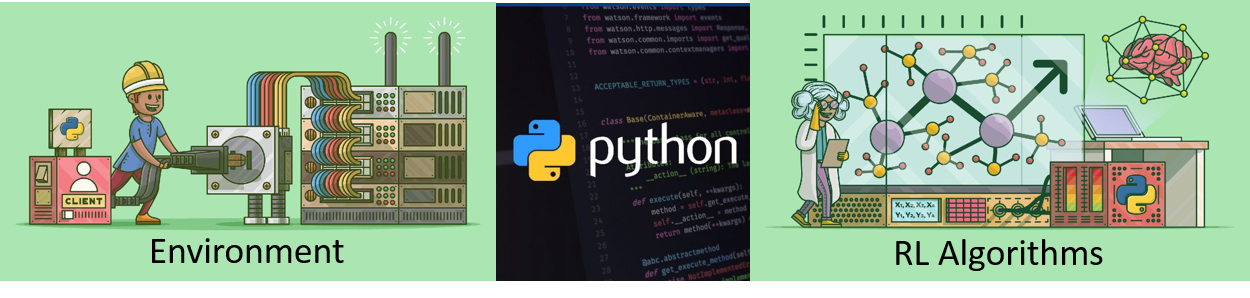
\includegraphics[width=\linewidth]{Figures/python-layers-env-alg}
	\caption{تقسیم بندی وظایف اصلی کد پایتون}
	\label{fig:python-layers-env-alg}
\end{figure}


دسته اول (سمت چپ تصویر
\ref{fig:python-layers-env-alg}
)
به پکیج های زیر احتیاج دارد:
\begin{multicols}{3}
\begin{itemize}
	\item \lr{numpy} \item \lr{socket} \item\lr{time} و \lr{os} \item \lr{pandas}
	\item \lr{matlab.engine} \item \lr{gym}
\end{itemize}
\end{multicols}
اگر از 
\glspl{w:anaconda}
برای پایتون استفاده می‌کنید غیراز دو بسته 
\lr{gym}
و 
\lr{matlab.engine}
به صورت پیش‌فرض نصب شده اند در صورت عدم نصب آن ها را با استفاده از 
\lr{pip}\RTLfootnote{مثلا بسته \lr{numpy} را با استفاده از دستور \lr{\texttt{pip install numpy}} نصب می‌توان کرد.}
می‌توان نصب کرد.

بسته \lr{gym} که در این فصل به‌تفصیل در مورد آن بحث شده است، به راحتی با همان دستور \texttt{pip} نصب می‌شود. اما نصب 
\lr{matlab.engine}
یا همان
\glspl{w:matlabengine}
متفاوت است و نمی‌توان آن را نیز به همان روش نصب کرد.

دسته دوم شامل بسته های زیر است:
\begin{itemize}
	\item \lr{gym[atari]} یا \lr{gym[all]}
	\item \lr{tensorflow}
	\item \lr{stable-baseline}
	
\end{itemize}

این بسته ها در لایه الگوریتم استفاده شده است.(در مورد این لایه در فصل 
\ref{ch:alg}
بیشتر صحبت خواهد شد.)
هر سه‌تای این بسته ها با همان دستور \lr{pip} به راحتی نصب می‌شوند.



\section{معرفی دقیق تر اجزای کلی}
در این قسمت میخواهیم سه نرم‌افزار کلی این پروژه را از نگاهی نزدیک تر  بشناسیم که عبارتند از :
\begin{enuminline}
	\item 
	نرم‌افزار 
	\glspl{w:prescan}
	\item 
	\glspl{w:matlab}
	\item پایتون
\end{enuminline}

\subsection{معرفی نرم‌افزار 
\glspl{w:prescan}
}

پس از دانلود و نصب نسخه \lr{8.5.0} این نرم‌افزار چهار آیکون مانند شکل 
\ref{fig:prescan-icons}
به محیط دسکتاپ اضافه می‌کند.  اصلی ترین آن ها 
\lr{PreScan Proccess Manager 8.5.0}
نام دارد.

\begin{figure}[h]
	\centering
	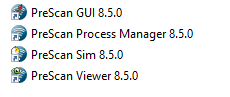
\includegraphics[width=0.4\linewidth]{Figures/prescan-icons}
	\caption{آیکون های اضافه شده بر روی محیط دسکتاپ پس از نصب پری‌اسکن}
	\label{fig:prescan-icons}
\end{figure}

با انتخاب آن صفحه ای مانند زیر باز می‌شود.

\begin{figure}[h]
	\centering
	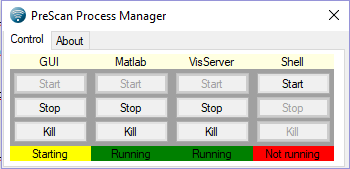
\includegraphics[width=0.5\linewidth]{Figures/Prescan-panel}
	\caption{پنل مدریت نرم‌افزار پری‌اسکن}
	\label{fig:prescan-panel}
\end{figure}

این پنجره شامل گزینه های زیر است:
\begin{multicols}{2}
	\begin{itemize}
		\item \lr{GUI}
		\item \lr{VisServer}
		\item \lr{Matlab}
		\item \lr{Shell}
	\end{itemize}
\end{multicols}

برای ایجاد یک محیط جدید باید \lr{GUI} را استارت کرد. پس از مدتی صفحه ای مانند شکل 
\ref{fig:prescan-gui}
باز می‌شود. 





\begin{figure}
	\centering
	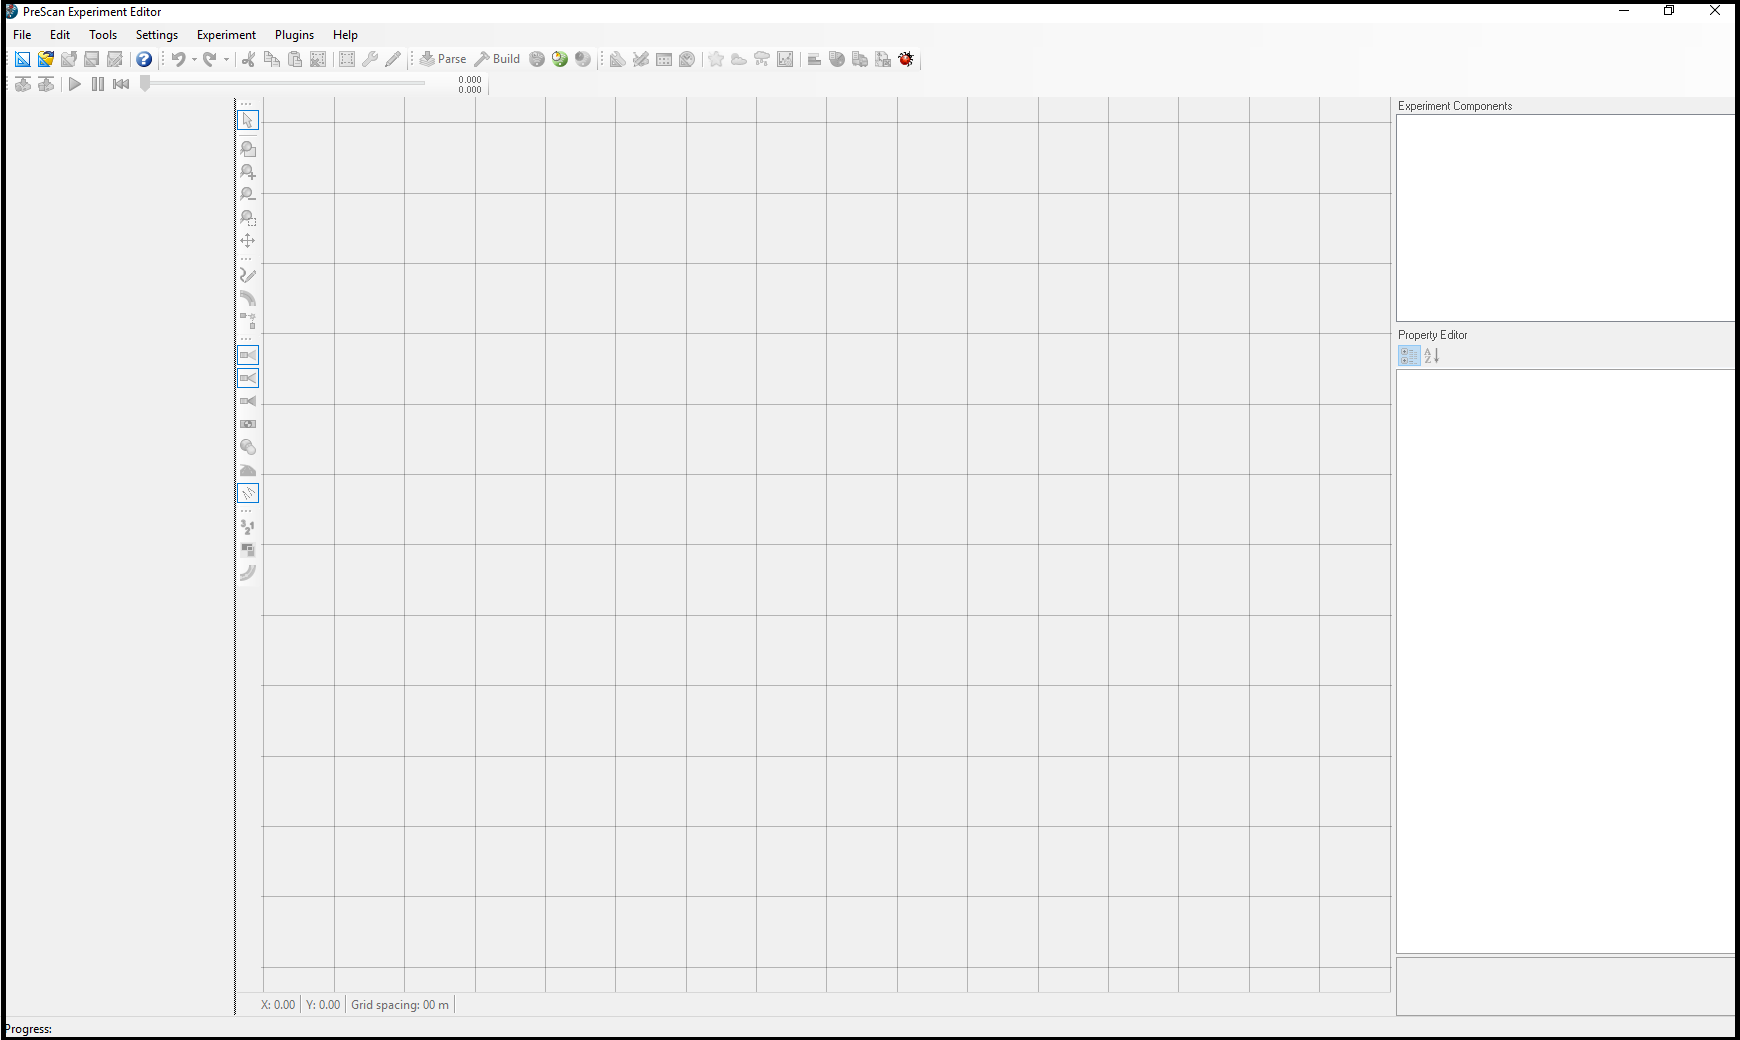
\includegraphics[width=0.7\linewidth]{Figures/Prescan-GUI}
	\caption{صفحه گرافیکی محیط پری‌اسکن}
	\label{fig:prescan-gui}
\end{figure}



پس از ایجاد مدل ها و ذخیره آن، فایل های \texttt{**.pex} و \texttt{**.pb} و \texttt{**\_cs.slx} ساخته می‌شود.
\RTLfootnote{علامت ** به معنای یک اسم مشترک در این سه فایل استفاده شده است. }

جهت استفاده از فایل سیمولینک باید در شکل 
\ref{fig:prescan-panel}
متلب را استارت کنید.
\begin{remark}
	برای اجرای فایل های سیمولینک خروجی، لازم است که متلب را فقط و فقط با استفاده از نرم افزار پری‌اسکن و با استفاده از پنل مدیریت نرم افزار معرفی شده در شکل 
	\ref{fig:prescan-panel}
	باز شود. در صورتی که به صورت مستقیم این کار انجام شود، به مشکل منتهی می‌شود.
\end{remark}


دو قسمت دیگر نیز در شکل 
\ref{fig:prescan-panel}
وجود دارد که نیازی به استارت کردن آن ها نیست و خودشان در صورت لزوم به صورت خودکار فراخوانی می‌شوند.

\subsection{فرمت های فایل های خروجی}
نرم‌افزار پری‌اسکن پس از ایجاد یک محیط جدید، فایل ها و پوشه های بسیار زیادی را ایجاد می‌کند. اما در خارج آن پوشه ها ۳ فایل وجود دارد که پسوند آن ها \texttt{**.pex} و \texttt{**.pb} و \texttt{**\_cs.slx} می‌باشد. علامت ** همان اسم پروژه‌ای است که ایجاد کرده ایم. هر یک از این فایل ها به یک بلوک از شکل 
\ref{fig:block-diagram}
مربوط می‌شود.

\begin{table}[h!]
	\tableset{
		%{\setcellgapes{0.5em}\makegapedcells
		\begin{tabular}{|C{0.15\linewidth}|p{0.8\linewidth}|}
			\hline\rowcolor{lightgray}
			فرمت فایل
			&
			توضیحات 
			\\\hline\hline
			\texttt{**.pex} &	این فایل مربوط به اولین بلوک شکل
			\ref{fig:block-diagram}
			است و ارتباط مستقیم با \lr{GUI} دارد. برای تغییر محیط گرافیکی باید این فایل را باز کرد.
			\\ \hline   
			\texttt{**.pb} & این فایل برخی از اطلاعات فایل 
			\texttt{**.pex}
			را در اختیار دارد و با تغییر آن فایل این فایل نیز عوض می‌شود. این فایل حاوی اطلاعات استاتیک محیط ایجاد شده است و مهم ترین کاربرد آن در بلوک موتور متلب که در شکل 
			\ref{fig:block-diagram}
			نشان داده شده است می‌باشد. پایتون از طریق این فایل این اطلاعات را دریافت می‌کند.
			\\\hline
			\texttt{**\_cs.slx} &
			این فایل سیمولینک است که برای کار کردن با آن باید از پنل مدیریت شکل
			\ref{fig:prescan-panel}
			استفاده کرد. این فایل پس از ایجاد از فایل 
			\texttt{**.pex}
			مستقل می‌شود. این فایل خود قابلیت تغییر دارد و می‌توان بلوک‌های آن‌را در محیط سیمولینک تغییر داد و بلوک های دیگری به آن افزود.  در صورتی که فایل \texttt{**.pex} تغییر کند، این امکان را نیز دارد که از داخل خود سیمولینک با فشردن دکمه ای این تغییرات جدید اعمال شود بدون آن که به تغییرات خود کاربر لطمه ای وارد شود. در این پروژه این فایل، تغییرات بسیاری را تجربه کرد.
			\\\hline
	\end{tabular}}
	\caption{توضیحات فرمت فایل خروجی}
	\label{tab:prescan-format}
\end{table}



جدول
\ref{tab:prescan-format}
توضیحات لازم را جهت آشنایی با این خروجی ها آورده است.

همچنین در بخش  
\ref{ch:fani|sec:simulink}
در مورد فایل \texttt{**\_cs.slx} توضیحات دقیق‌تری در مورد جزییات آن گفته خواهد شد.





\subsection{نصب
\glspl{w:matlabengine}
}
برای نصب موتور متلب ابتدا نیاز است که به متلب به طور کامل در سیستم نصب باشد. پس از نصب متلب، محیط \lr{Command prompt (admin)} را باز کنید و با توجه به نسخه و محل نصب متلب خود به آدرس زیر بروید.

\begin{center}
	\LRE{\verb|<matlabroot>\extern\engines\python|}
\end{center}

مثلا برای \lr{Matlab R2017b} که در محل پیش‌فرض خود نصب شده باشد این کار با استفاده از دستور زیر انجام می‌شود.

\begin{center}
	\LRE{\verb|cd C:\Program Files\MATLAB\R2017a\extern\engines\python|}
\end{center}

در این پوشه یک فایل به نام \lr{setup.py} موجود می‌باشد. این فایل را با استفاده از دستور 

\begin{center}
	\LRE{\verb|python setup.py install|}
\end{center}

در همان محیط \lr{cmd} اجرا کنید.

\begin{note}
	توجه داشته باشید که باید نسخه متلب و پایتون شما باید با یکدیگر سازگار باشند. برای بررسی این موضوع اگر فایل \lr{setup.py} را با اسنفاده از یک ادیتور باز کنید، یک آرایه به نام \texttt{\_supported\_versions} در آن خواهید دید. مقادیر این آرایه، نسخه هایی از پایتون را نشان می‌دهد که توصط نسخه متل شما پشتیبانی میشود مثلا در این مورد، با توجه به خط زیر نسخه های $2.7$ ، $3.4$ ، $3.5$ و $3.6$ پاینون پشتیبانی می‌شود. در غیر این صورت باید نسخه سازگار متلب و یا پایتون را نصب کنید.
	\begin{center}
		\lr{\texttt{\_supported\_versions = ['2.7', '3.4', '3.5', '3.6']}}
	\end{center}
\end{note}

\section{معرفی دقیق تر پیشنیاز های پایتون}
\subsection{بسته‌های کمکی}
این بسته ها نقش حیاتی ندارند و برای برخی از موارد استفاده شده‌اند. این موارد در جدول
\ref{table:aux-packages}
آمده است.

\begin{table}[t!]\tableset{
	\begin{tabular}{|C{0.13\linewidth}|C{0.52\linewidth}|C{0.25\linewidth}|}
		\hline\rowcolor{lightgray} نام بسته  &  دلیل استفاده & روش نصب
		\\\hline
		\lr{numpy} & ایجاد ماتریس برای \glspl{w:actionspace} و \glspl{w:obsspace} & \LRE{\texttt{pip install numpy}}
		\\\hline
		\lr{time} & جهت ایجاد تاخیر و 
		\glspl{w:timeout}
		 & \LRE{\texttt{pip install time}}
		\\\hline
		\lr{os} & برای بستن پنجره های باز شده پس از اجرا & \LRE{\texttt{pip install os}}
		\\\hline
		\lr{pandas} & برای چاپ اطلاعات آماری 
		\glspl{w:reward}
		های بدست آمده در پایان هر 
		\glspl{w:episode}
		 & \LRE{\texttt{pip install pandas}}
		\\\hline
		\lr{socket} & برقراری ارتباط با 
		\w{matlab}
		و فرستان و دریافت کردن 
		\ws{dyndata}
		 & \LRE{\texttt{pip install socket}}
		\\\hline
		\lr{tensorflow} & برای لایه الگوریتم و استفاده از الگوریتم‌های
		\w{drl}
		 & \LRE{\texttt{pip install tensorflow}}
		\\\hline
	\end{tabular}}
	\caption{}
	\label{table:aux-packages}
\end{table}

\subsection{بسته \lr{gym}}

\subsubsection{معرفی}
بسته 
\href{https://github.com/openai/gym}{\lr{gym}}
 که توسط 
 \href{https://github.com/openai}{\lr{OpenAI}}
 توسعه یافته است. این ابزار فوق العاده این امکان را برای محقیقین علوم کامپیوتر حرفه‌ای و یا آماتور فراهم می‌کند که انواع الگوریتم های 
 \w{rl}
 (\gls*{a:rl})
 را بر روی کار خود تست کنند. همچنین پتانسیل این را دارد که محقیقن محیط خود را برروی این بسته توسعه دهند.
 
 هدف از ایجاد این بسته، استاندارد سازی 
\w{env}
و نوعی 
\w{benchmark}
برای پژوهش های 
\gls*{a:rl}
محسوب می‌شود.\cite{medgyminstall}

در حقیقت می‌توان این بسته را در وسط شکل
\ref{fig:python-layers-env-alg}
جای‌ داد. جایی که لایه 
\w{env}
و لایه 
\w{alg}
به‌یک‌دیگر می‌رسند. 

 این بسته محیط هایی از پیش ساخته شده دارد. نام این بسته ها در لیست زیر
 آمده است. 
 \RTLfootnote{جدول کامل در سایت 
 	\url{https://github.com/openai/gym/wiki/Table-of-environments}
قرار دارد. 
}
 اکثر این محیط ها نوعی بازی هستند که 
 \w{agent}
 سعی در یادگیری آن محیط ها دارد.

 
\begin{multicols}{2}\scriptsize\setstretch{0.5}
\begin{itemize}
\item \lr{CartPole-v0}
\item \lr{Pendulum-v0}
\item \lr{MountainCar-v0}
\item \lr{MountainCarContinuous-v0}
\item \lr{BipedalWalker-v2}
\item \lr{Humanoid-V1}
\item \lr{Riverraid-v0}
\item \lr{Breakout-v0}
\item \lr{Pong-v0}
\item \lr{MsPacman-v0}
\item \lr{SpaceInvaders-v0}
\item \lr{Seaquest-v0}
\item \lr{LunarLanderV2}
\item \lr{Reacher-v2}
\item \lr{FrozenLake-v0}
\end{itemize}
\end{multicols}


% OpenAI Gym is an awesome tool which makes it possible for computer scientists, both amateur and professional, to experiment with a range of different reinforcement learning (RL) algorithms, and even, potentially, to develop their own.

%Built with the aim of becoming a standardized environment and benchmark for RL research, OpenAI Gym is a Python package comprising a selection of RL environments, ranging from simple “toy” environments, to more challenging environments, including simulated robotics environments and Atari video game environments.
\subsubsection{نصب}
 برای نصب نسخه کمینه این نرم افزار با همان روش \lr{pip} به راحتی می‌توان نرم‌افزار مورد نظر را نصب کرد.
 \cite{git/gym}
 این نسخه کمینه برای لایه 
 \w{env}
 کافی می‌باشد. اما اگر بخواهیم بخش \w{alg} را با استفاده از کتابخانه های دیگری مانند \lr{stable-baseline} نوشت. نیازمند نسخه جامع تری از \lr{gym} می‌باشد.

\begin{note}
پیشنهاد می‌شود برای نصب نسخه کامل \lr{gym} و \lr{stable-baseline} از لینوکس بجای ویندوز استفاده کنید. زیرا در نصب برخی بسته ها ممکن است با مشکل روبرو شوید.
\end{note}

برای نصب کامل این بسته از دستور \LRE{\texttt{pip install gym[all]}} را استفاده کنید. ممکن است در نصب \lr{mujuco} به مشکل برخورید در این صورت دستور \LRE{\texttt{pip install gym[atari]}} استفاده کنید.

اگر موفق به نصب این بسته نشدید می‌توانید مراجل نصب آن را با استفاده از 
\cite{medgyminstall}
مراجعه کنید.